\newlength{\centeroffset}
\setlength{\centeroffset}{-0.5\oddsidemargin}
\addtolength{\centeroffset}{0.5\evensidemargin}
%\addtolength{\textwidth}{-\centeroffset}
\thispagestyle{empty}
\vspace*{\stretch{1}}
\noindent\hspace*{\centeroffset}\begin{minipage}{\textwidth}
\flushright
{\Huge\bfseries
  La Riera Blanca:\\una frontera invisible?

}
\noindent\rule[-1ex]{\textwidth}{5pt}\\[4.5ex]

\begin{center}
      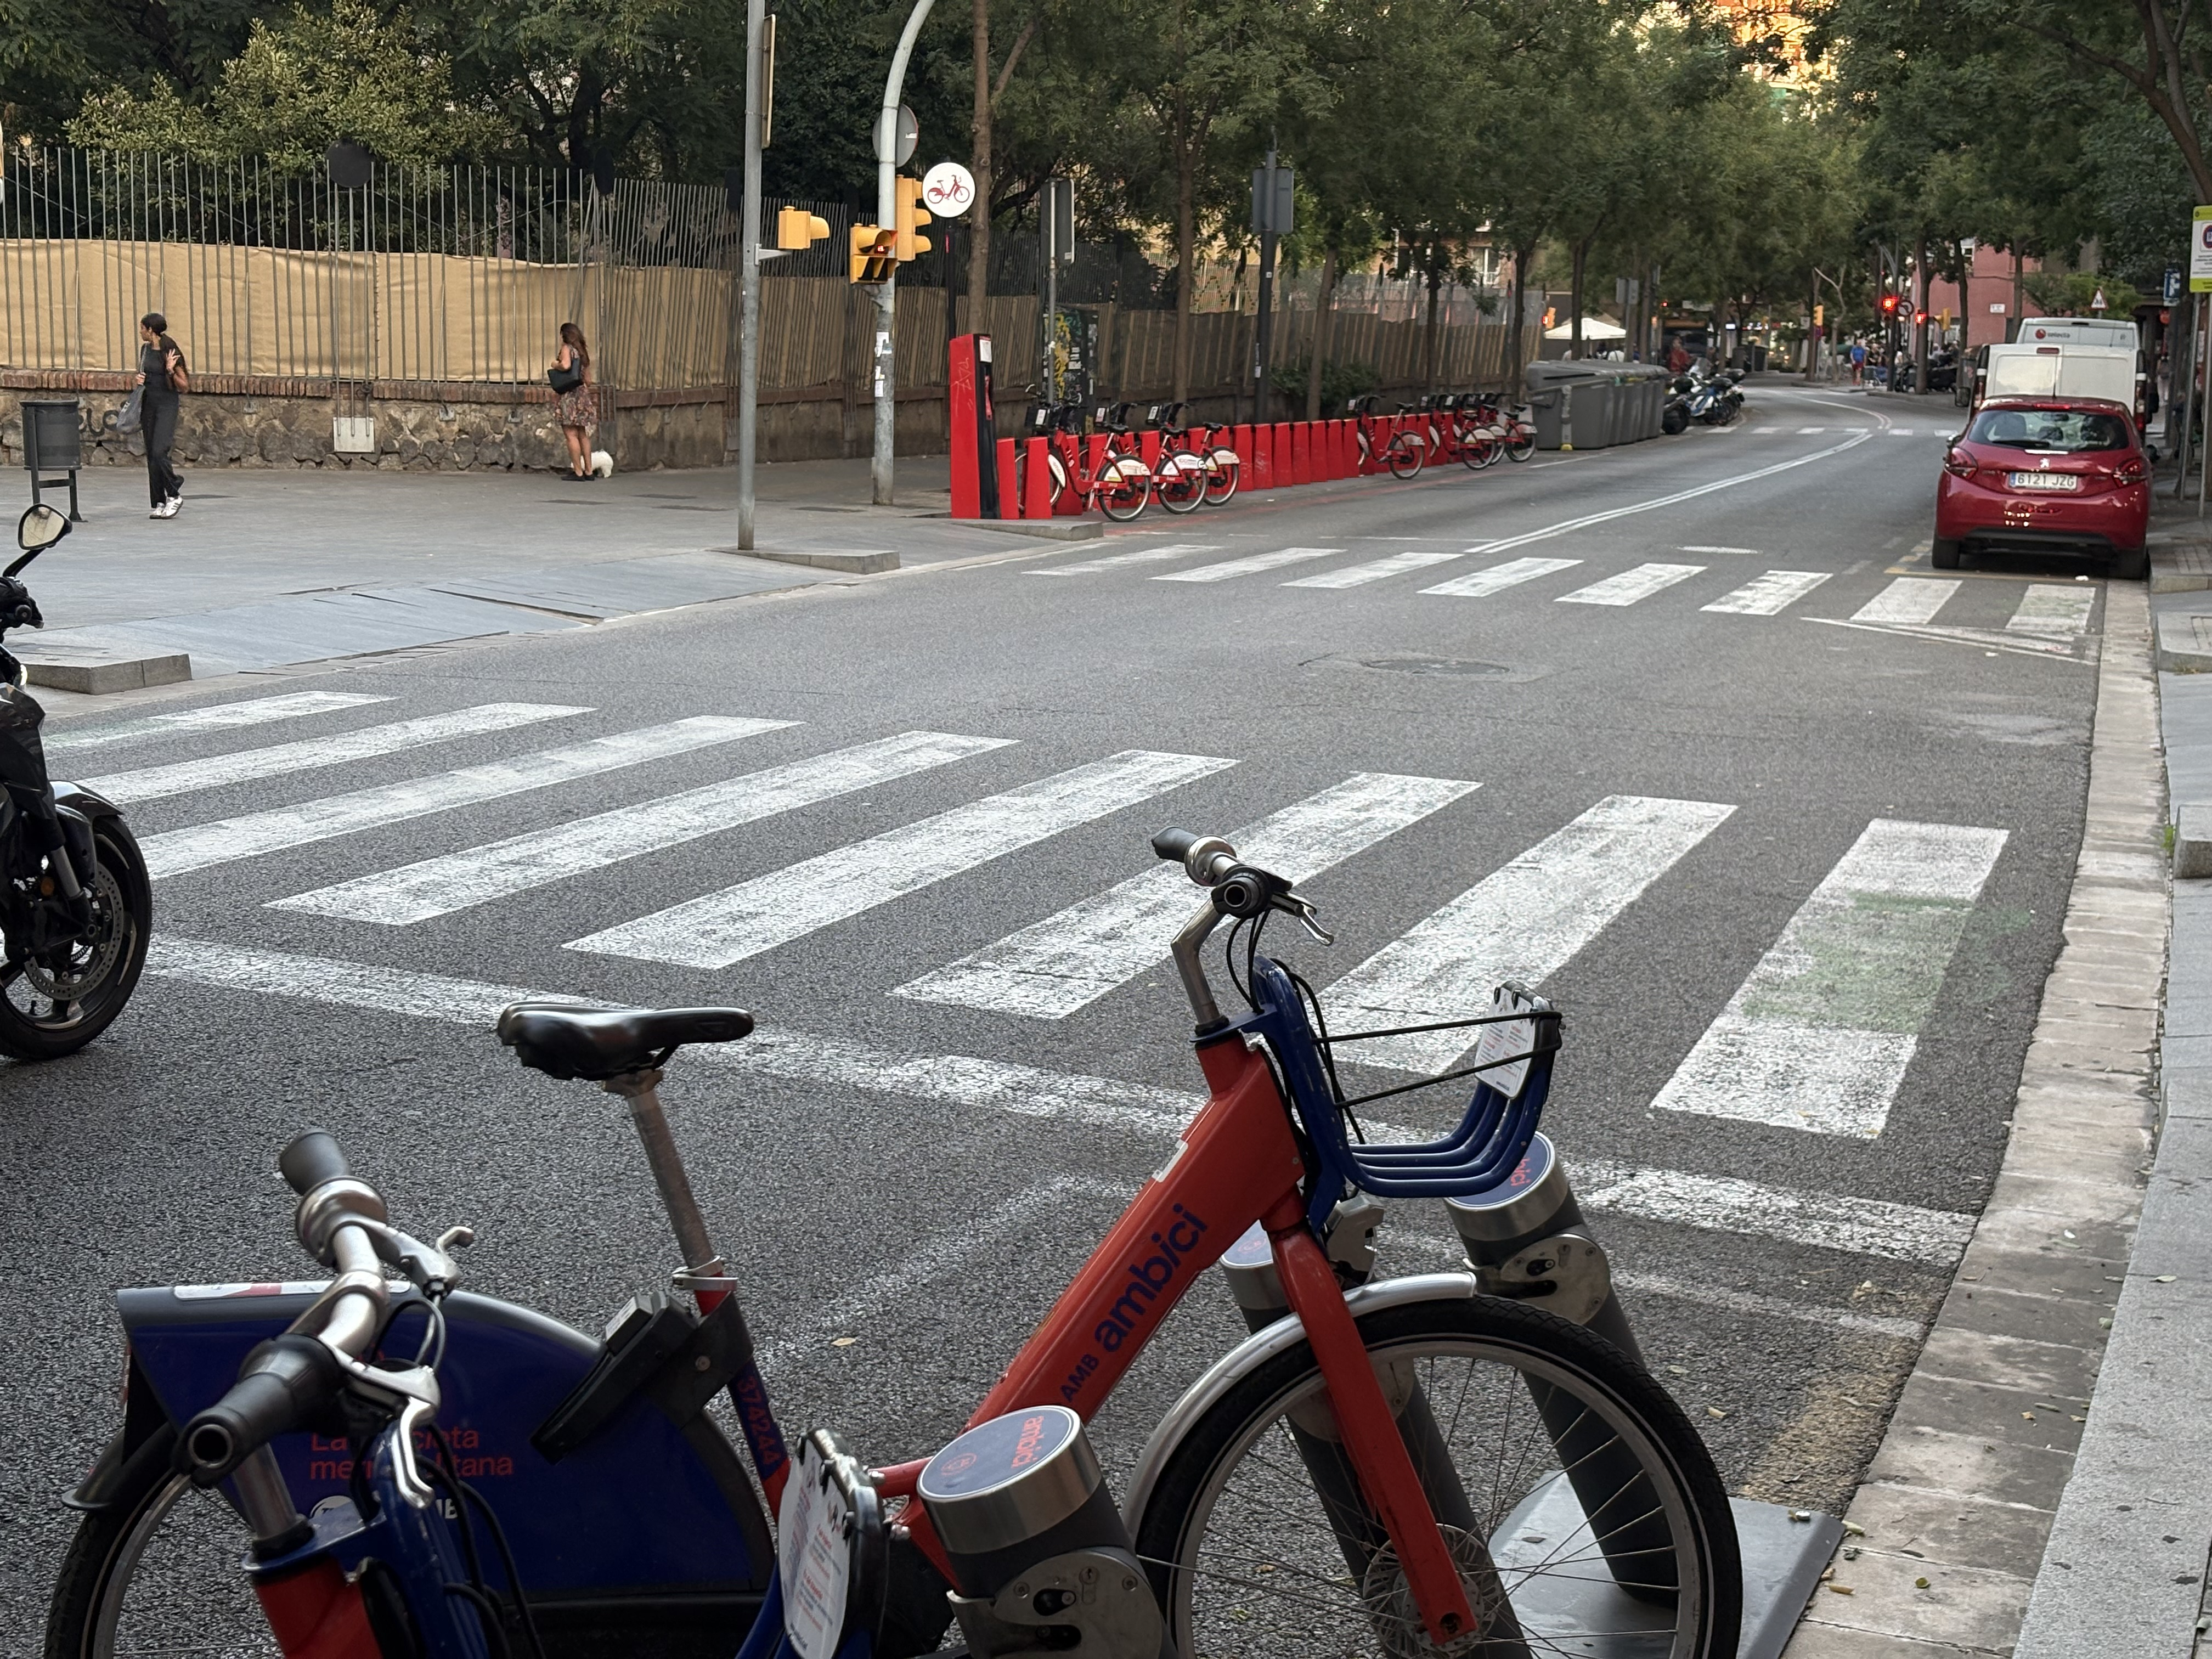
\includegraphics[width=0.6\textwidth]{./imatges/portada.jpeg}
\end{center}
\vspace*{3truecm}


\end{minipage}

\vspace{\stretch{1}}
\noindent\hspace*{\centeroffset}\begin{minipage}{\textwidth}
\flushright
{\bfseries 
	Max Pérez Sastre\\}
	Tutor: Fernando García Vílchez\\
	Departament de Matemàtiques\\
	Institut Sants\\
	\today

\end{minipage}
%\addtolength{\textwidth}{\centeroffset}
\vspace{\stretch{2}}


\pagebreak
\thispagestyle{empty}

\vspace*{16truecm}

	\begin{quote}
	\textbf{Avís legal}

	  Copyright \copyright{} Max Pérez Sastre.
	  Es garanteix permís per copiar, distribuir i modificar aquest document segons els termes de la GNU Free Documentation License, versió 1.3 o qualsevol posterior publicada per la Free Software Foundation. Es disposa d'una còpia d'aquesta llicència a~\href{http://www.fsf.org}{http://www.fsf.org} i a l'annex~\ref{a:license}.
	\end{quote}



\endinput
